\section{Hardware}
\label{sec:hw}

In this section hardware used in the process of creating capture device is described, system schematic is laid out whilst taking into account the hardware limitations of chosen hardware, namely the focal length and depth of field of the chosen lens.

\subsection{Hardware Setup}
To be able to effectively scan 2D biometry of hand various hardware is necessary. Firstly we need structure to hold all other hardware together robust enought to hold weight and absorb vibrations generated by rail. This requirement is satisfied by using an aluminium framework.

Rail itself is mounted on this framework in a way to allow slide to move freely above the hand position. Camera and light are mounted on the slide moving along the rail to allow continuous capture of hand geometry with best lightning conditions.
Control module consists of Raspberry Pi 3 and Arduino UNO running software necessary for capturing hand geometry and controlling the slide rail.
\begin{figure}[ht!]
    \label{fig:setup}
    \centering
    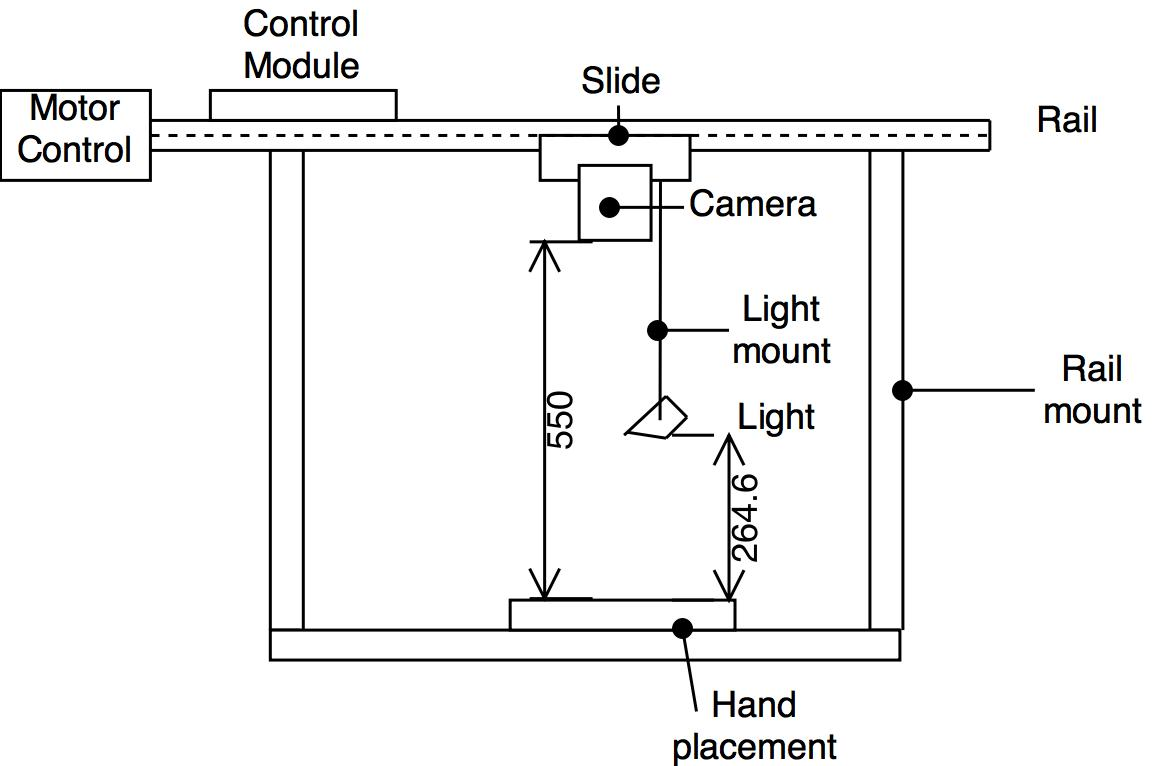
\includegraphics[width=0.75\linewidth]{setup.jpg}
    \caption{Schematic of hardware setup.}
\end{figure}

%\begin{figure}[ht]
%    \label{fig:overview}
%    \centering
%    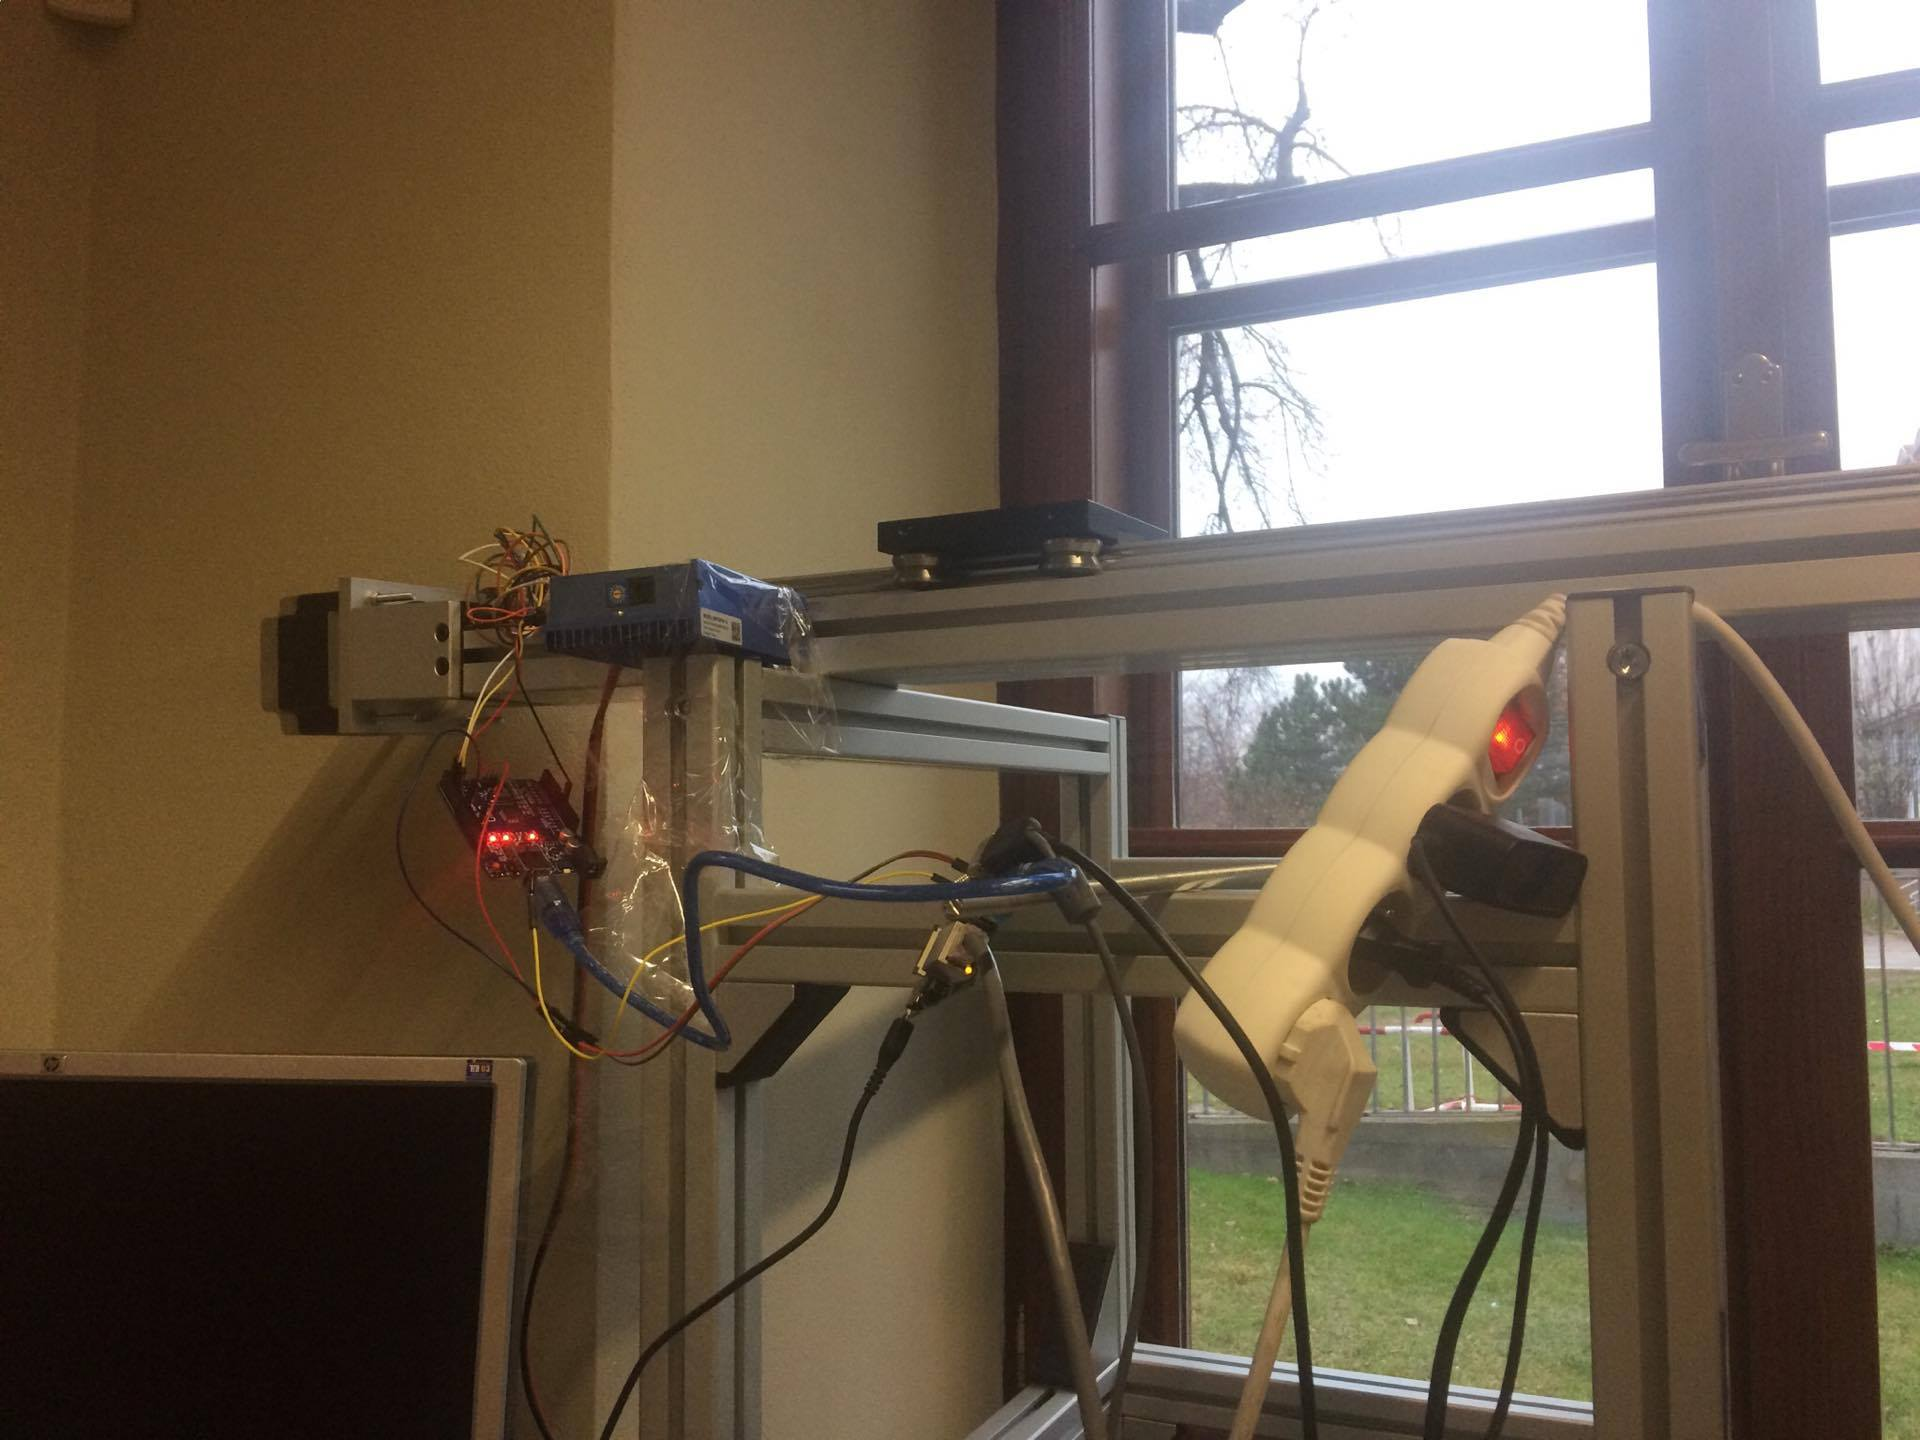
\includegraphics[width=0.75\linewidth]{overview.jpg}
%    \caption{Hardware Setup.}
%    \todo[inline]{nova foto}
%\end{figure}

\subsubsection*{Camera}
The selected camera is Basler raL6144-16gm. This camera provides us with the resolution of 6144 $\times$ 1 pixels with line rate up to 17 kHz and is controlled via ethernet connection and Pylon SDK.
The captured image is in greyscale colors. The camera's shutter can be operated either via hardware or software trigger\footnote{The camera also enables "free-run mode".}.

The camera is equipped with AF Nikon 50 mm f1.8D lens. The lens suits our needs for multiple reasons:
It is relatively inexpensive, simple to use and has good depth-of-field control with aperture ranging from f/1.8 up to f/22.

\subsubsection*{Camera Mount}
In order to acquire images with line camera either scanned object or camera have to move in smooth direct line to cover the whole scanned area.
We decided to move with the camera because in order to minimize errors during scanning. The scanned hand is placed on stable platform and with only camera mount moving,
human error is minimized and user experience is improved.

Slide moving along the rail houses the platform where the camera is mounted. This platform is facing down with camera and light mounted as seen in figure \ref{fig:camera-mount}.

\begin{figure}[ht]
    \label{fig:camera-mount}
    \centering
    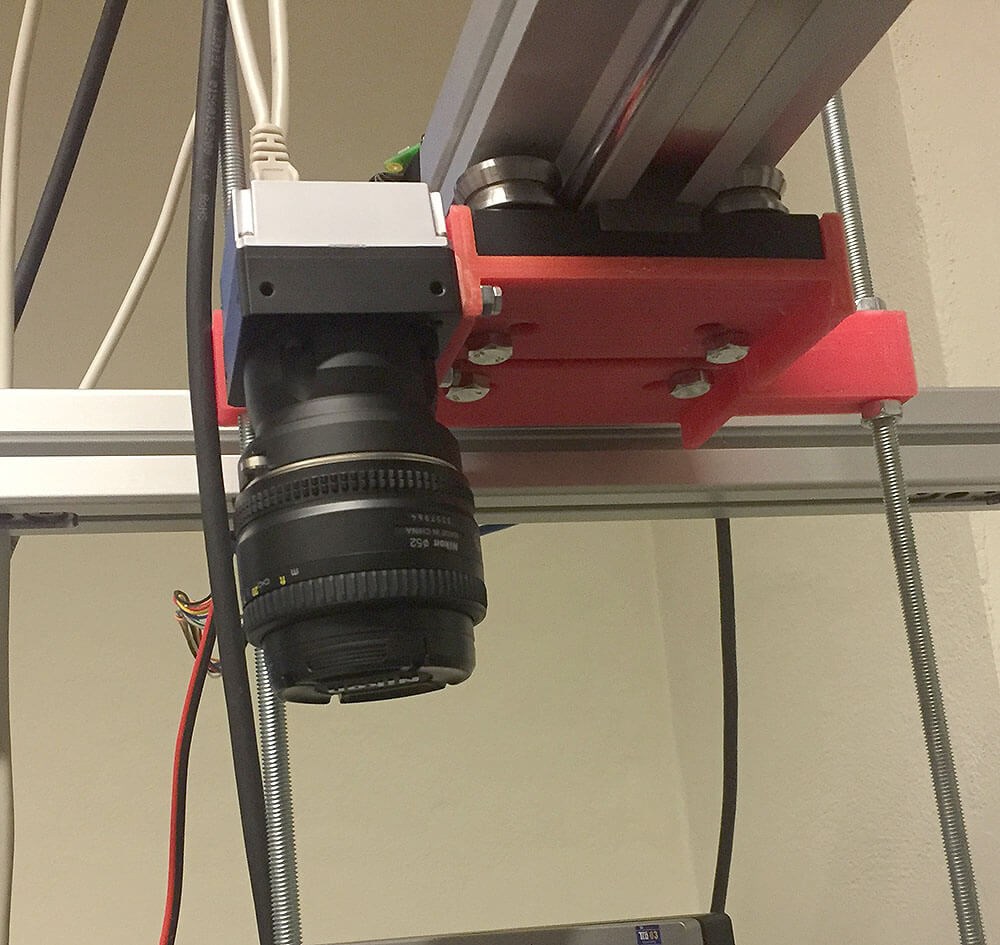
\includegraphics[width=0.5\linewidth]{camera-mount.jpg}
    \caption{camera mount setup}
\end{figure}


\subsubsection*{Slide Rail \& Stepper Motor}
Slide moves on the rail in uniform motion along the rail axis. Slide movement is controlled by a stepper motor which controls direction and speed of the movement.
Rail is mounted on the framework in the height of 60 cm. This allows us to a fine-tune the focus point of both the camera and the light.
\todo[inline]{Preco je to v danej vyske, vypocet vysky}

The stepper motor itself is controlled by Leadshine EM705 Digital Stepper Drive which is controlled by pulses. We generate pulse width modulation (PWM) generated by Arduino UNO with our custom code generating 62 500 Hz PWM with 50 \% duty cycle in Fast PWM mode.

The PWM can be calculated as follows:

${PWM}_{Frequency} = 16000000 / (Prescale\_Factor * 256)$

where $Prescale\_Factor$ can be set to 1, 8, 64, 256 or 1024. The default value is 64. Our code utilizes the Timer 2 available on Arduino UNO with prescale factor set to 1 which results in aforementioned 62 500 Hz PWM.

Apart from the PWM the Arduino UNO specifies in which direction the stepper motor should operate. The Leadshine EM705 Digital Stepper Drive also makes available the \texttt{ENABLE} signal which enables the output from it.

\subsection{Slide Rail Control}
\label{sec:serial}
The Arduino UNO itself is controlled via the serial interface where it actively listens for incoming messages. We defined a simple protocol:
\begin{verbatim}
<L|R><0 - 99999>
\end{verbatim}
where the first characted specifies the direction of the movement. \texttt{L} stands for leftward movement which moves the slide towards the base of the rail. \texttt{R} standing for rightward movement move the slide away from the stepper motor.

After the direction specification follows the duration stated in miliseconds of the movement. One milisecond of movement equals to XX mm as calculated by following formula:
\todo[inline]{Vypocet rychlosti v mm/ms}

The Arduino UNO is connected to the Raspberry Pi 3 via USB which serves as the serial port and as power source at once. The serial interface is set to the baud rate of 115 200 baud/s.

The Raspberry Pi 3 then sends messages in format specified in \ref{sec:serial} and doesn't wait for any response since Arduino UNO serves as a standalone module and the Arduino UNO's output is only for debugging and informative purposes. Other options such as generating PWM directly on Raspberry Pi 3 or controlling Arduino UNO via GPIO pins were considered but during the development we stumbled upon problems with consistent and smooth signal generation caused by Raspberry Pi 3 itself which is not suited for such applications.

\subsection{Light}
To acquire high quality images of hand it is necessary to have proper light source. The line light chosen for our assignment is Chromasens Corona II type C with LED-control unit XLC4-1 which can produce up to 300 000 lux. The light is mounted directly below the slide platform is angled at 10 $^{\circ}$ towards camera's line of sight.

LED-Control unit is controlled through the telnet interface via which one can set light intensity, set channels on or off and query various metrics and information. The LED-Control unit has a default IP address \texttt{192.168.87.234} and default credentials with username \texttt{admin} and password \texttt{chromasens}. We provide a simple interface for interacting with the control unit via a script \texttt{rail-control/tel\_commander.py}.

\subsection{Hand Placement}
The hand is placed in the centre of the framework on a prepared platform which aligns and spreads the fingers in order to
capture the same hand geometry during different scans. The hand is stable during image capture procedure which minimizes human error.
Figure \ref{fig:hand-placement} shows placement of hand during scan.

\begin{figure}[ht]
    \label{fig:hand-placement}
    \centering
    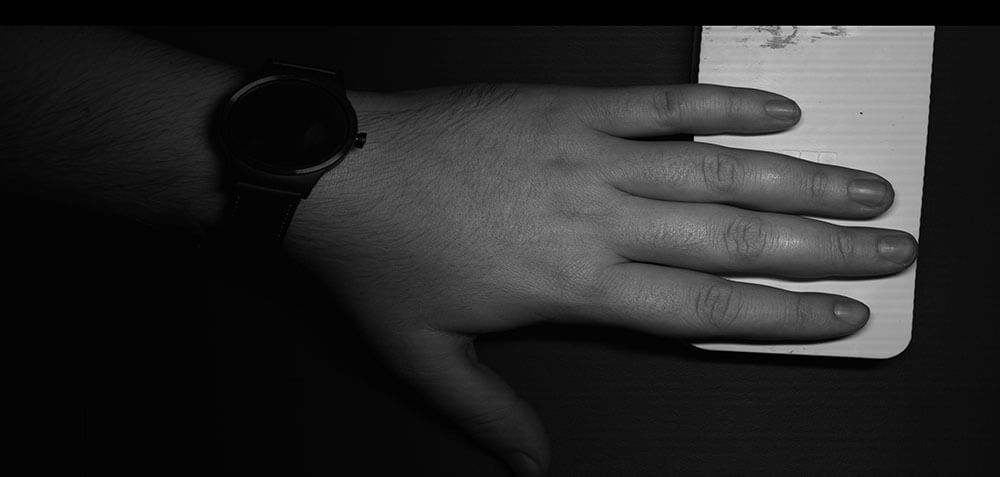
\includegraphics[width=0.8\linewidth]{hand-top.jpg}
    \caption{Hand placement during scan}
    \todo[inline]{zmenit/orezat foto}
\end{figure}

\subsection{Control}
The whole system is connected via ethernet with a router which is setup up to assign IPs from \texttt{192.168.87.1/28} because of the default configuration of the LED-control unit. User enters the system through the Raspberry Pi 3 and issues commands on it with a prepared script \texttt{rail-control/capture.py}.

